\documentclass[]{standalone}

\usepackage{graphicx}
\usepackage[linesnumbered,ruled,vlined]{algorithm2e}
\usepackage{color,soul}
\usepackage[utf8]{inputenc}
\usepackage[T1]{fontenc}
\usepackage{textcomp}
\usepackage{amsmath, amssymb}
\usepackage{caption}
\usepackage{listings}

% figure support
\usepackage{tikz}
\usetikzlibrary{calc}
\usepackage{import}
\usepackage{xifthen}
\pdfminorversion=7
\usepackage{pdfpages}
\usepackage{transparent}
\usepackage[hidelinks]{hyperref}

\pdfsuppresswarningpagegroup=1

\begin{document}
	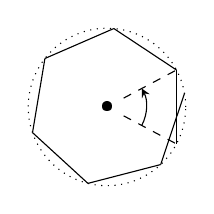
\begin{tikzpicture}[>=stealth]
		\node[] (Robot) at (0,0) {\textbullet};
		
		\draw[dashed] (Robot) -- ($(Robot)+(-28:1)$);
		\draw[dashed] (Robot) -- ($(Robot)+(+28:1)$);
		\draw ($(Robot)+(-28:1)$)--($(Robot)+(28:1)$);
		\draw ($(Robot)+(28:1)$)--($(Robot)+(85:1)$);
		\draw ($(Robot)+(85:1)$)--($(Robot)+(142:1)$);
		\draw ($(Robot)+(142:1)$)--($(Robot)+(199:1)$);
		\draw ($(Robot)+(199:1)$)--($(Robot)+(256:1)$);
		\draw ($(Robot)+(256:1)$)--($(Robot)+(313:1)$);
		\draw ($(Robot)+(313:1)$)--($(Robot)+(370:1)$);
		\draw[->] ($(Robot)+(-28:0.5)$) arc (-28:28:0.5);
		\draw[dotted] (Robot) circle[radius=1];
		
	\end{tikzpicture}
\end{document}
